\documentclass[final]{beamer}
%% Possible paper sizes: a0, a0b, a1, a2, a3, a4.
%% Possible orientations: portrait, landscape
%% Font sizes can be changed using the scale option.
\usepackage[size=a0,orientation=portrait]{beamerposter}

\usetheme{gemini}
\usecolortheme{seagull}
\useinnertheme{rectangles}

% ====================
% Packages
% ====================

\usepackage[utf8]{inputenc}

\usepackage{graphicx}
\usepackage{booktabs}
\usepackage{tikz}
\usepackage{pgfplots}
\usepackage{wrapfig,lipsum}
\usepackage{cleveref}


% \usepackage{sidecap}

% ====================
% Lengths
% ====================

% If you have N columns, choose \sepwidth and \colwidth such that
% (N+1)*\sepwidth + N*\colwidth = \paperwidth
\newlength{\sepwidth}
\newlength{\colwidth}
\setlength{\sepwidth}{0.02\paperwidth}
\setlength{\colwidth}{0.47\paperwidth}
% \setlength\abovecaptionskip{-5pt}
\setlength\belowcaptionskip{-5pt}
\setlength{\headsep}{-5pt}

\newlength{\sepparagraph}
\setlength{\sepparagraph}{0.5em}

\newcommand{\separatorcolumn}{\begin{column}{\sepwidth}\end{column}}
\newcommand{\sepnewparagraph}{\vspace{\sepparagraph}}

% ====================
% Logo (optional)
% ====================

% LaTeX logo taken from https://commons.wikimedia.org/wiki/File:LaTeX_logo.svg
% use this to include logos on the left and/or right side of the header:
\logoright{
\includegraphics[height=6cm]{logos/nju_logo.png}}
\logoleft{
\includegraphics[height=6cm]{logos/nju_logo.png}}

% ====================
% Footer (optional)
% ====================

% \footercontent{
% 	AERSS Conference 2023, Wuhan, China \hfill
% 	\insertdate \hfill
% 	\href{mailto:myemail@exampl.com}{\texttt{juhaoxing@qq.com}}
% }
% (can be left out to remove footer)

% ====================
% My own customization
% - BibLaTeX
% - Boxes with tcolorbox
% - User-defined commands
% ====================
% ====================
% BibLaTeX
% ====================

\usepackage[backend=biber,
	bibstyle=authoryear,
	citestyle=authoryear,
	style=authoryear,
	maxcitenames=2,
	maxbibnames=20, % limit the length of list of names (authors/editors/etc.)
	sorting=ydnt, % sort references by year (descending), name, title
	dashed=false, % show authors instead of dash in publications having the same authors
	giveninits=true % render authors' given name initials and not the full given names
]{biblatex}
%% Biblatex with Beamer bibliography icons
\setbeamertemplate{bibliography item}{%
	\ifboolexpr{ test {\ifentrytype{book}} or test {\ifentrytype{mvbook}}
		or test {\ifentrytype{collection}} or test {\ifentrytype{mvcollection}}
		or test {\ifentrytype{reference}} or test {\ifentrytype{mvreference}} }
	{\setbeamertemplate{bibliography item}[book]}
	{\ifentrytype{online}
		{\setbeamertemplate{bibliography item}[online]}
		{\setbeamertemplate{bibliography item}[article]}}%
	\usebeamertemplate{bibliography item}}
\defbibenvironment{bibliography}
{\list{}
	{\settowidth{\labelwidth}{\usebeamertemplate{bibliography item}}%
		\setlength{\leftmargin}{\labelwidth}%
		\setlength{\labelsep}{\biblabelsep}%
		\addtolength{\leftmargin}{\labelsep}%
		\setlength{\itemsep}{\bibitemsep}%
		\setlength{\parsep}{\bibparsep}}}
{\endlist}
{\item}
%% Redefine \refname
\renewcommand{\bibname}{References}
%% Redefine \parencite to use square brackets instead of braces
\DeclareCiteCommand{\parencite}
{\usebibmacro{prenote}}
{\usebibmacro{citeindex}%
	\printtext[bibhyperref]{[\usebibmacro{cite}]}}
{\multicitedelim}
{\usebibmacro{postnote}}
%% Highlight author names using Beamer data annotation
%% Usage: add a new line `author+an = {<author-order>=highlight}` to an entry
%% For example: author+an = {3=highlight} => highlight the 3rd author name
\AtBeginBibliography{
	\renewcommand*{\mkbibnamegiven}[1]{%
		\ifitemannotation{highlight}
		{\textbf{#1}}
		{#1}%
	}
	
	\renewcommand*{\mkbibnamefamily}[1]{%
		\ifitemannotation{highlight}
		{\textbf{#1}}
		{#1}%
	}
}


% ====================
% Boxes with tcolorbox
% ====================
\usepackage[most]{tcolorbox}

%%% Beamer colors in boxes

\newcommand{\beamercolorsinboxes}[1]{
	\setbeamercolor{itemize item}{fg=#1!75!black}
	\setbeamercolor{itemize/enumerate body}{fg=#1!65!white}
	\setbeamercolor{itemize/enumerate subbody}{fg=#1!65!white}
	\setbeamercolor{item projected}{fg=white, bg=#1!75!black}
}

%%% Highlight Oval Box
\newtcbox{\xmybox}[1][red]{on line,
	arc=7pt,colback=#1!10!white,colframe=#1!50!black,
	before upper={\rule[-3pt]{0pt}{10pt}},boxrule=1pt,
	boxsep=0pt,left=6pt,right=6pt,top=2pt,bottom=2pt}
%%% Box for stating problems
%%%%%%%%
%Usage: (similar for infobox)
%	\begin{defbox}{title}
	%		contents
	%	\end{defbox}
%%%%%%%%
\newtcolorbox{defbox}[1]{%
	enhanced,
	attach boxed title to top 	left={xshift=5mm,yshift=-5mm,yshifttext=-5mm},
	colback=cyan!5!white,
	colframe=cyan!75!black,
	coltitle=cyan!80!black,
%	left=0mm,right=0mm,top=2mm,bottom=0mm,
	title={#1},
	fonttitle=\bfseries\large, fontupper=\color{cyan!65!white},
	boxed title style={colback=cyan!5!white,colframe=cyan!75!black},
	before upper={
		\beamercolorsinboxes{cyan}
	}
}%
%%% Box for announcement
\newtcolorbox{infobox}[1]{%
	enhanced,
	attach boxed title to top 	left={xshift=5mm,yshift=-5mm,yshifttext=-5mm},
	colback=yellow,
	colframe=red!75!black,
	coltitle=red!75!black,
%	left=0mm,right=0mm,top=2mm,bottom=0mm,
	title={#1},
	fonttitle=\bfseries\large, fontupper=\color{red!65!white},
	boxed title style={colback=yellow,colframe=red!75!black},
	before upper={
		\beamercolorsinboxes{red}
	}
}%
%%% Box for example
\newtcolorbox{exabox}[1]{%
	enhanced,
	attach boxed title to top 	left={xshift=5mm,yshift=-5mm,yshifttext=-5mm},
    colback=brown!5!white,
    colframe=brown!75!black,
    coltitle=black,
%	left=0mm,right=0mm,top=2mm,bottom=0mm,
	title={#1},
	fonttitle=\bfseries\large, fontupper=\color{black},
	boxed title style={colback=brown!5!white,coltitle=brown!50!brown!75!black},
	before upper={
		\beamercolorsinboxes{brown}
	}
}%
%%% Theorem Box
%%%%%%%%
%Usage: (similar for conjecture, lemma, etc.)
%	\begin{thm}{title}{nameref}
	%		contents
	%	\end{thm}
% Use \ref{thm:nameref} to refer to the theorem
%%%%%%%%
%%%% Use \newtcbtheorem[number within=section]{thm} to number within each section
\newtcbtheorem[]{thm}%
{Theorem}{attach boxed title to top 	left={xshift=5mm,yshift=-5mm,yshifttext=-5mm},
	enhanced jigsaw,
	%	top=2mm,bottom=0mm,left=0mm,right=0mm,
	fonttitle=\bfseries\large,fontupper=\itshape\color{blue!65!white},
	colframe=blue!75!black,colback=blue!5!white,coltitle=blue!50!blue!75!black,
	boxed title style={colback=blue!5!white,coltitle=blue!50!blue!75!black},
	before upper={
		\beamercolorsinboxes{blue}
	}
}{thm}%
%%% Proposition Box
\newtcbtheorem[use counter from=thm]{prop}%
{Proposition}{attach boxed title to top 	left={xshift=5mm,yshift=-5mm,yshifttext=-5mm},
	enhanced jigsaw,
	%	top=2mm,bottom=0mm,left=0mm,right=0mm,
	fonttitle=\bfseries\large,fontupper=\itshape,
	colframe=gray!75!black,colback=gray!5!white,coltitle=gray!50!gray!75!black,
	boxed title style={colback=gray!5!white,coltitle=gray!50!gray!75!black},
	before upper={
		\beamercolorsinboxes{gray}
	}
}{prop}%
%%% Conjecture Box
\newtcbtheorem[use counter from=thm]{conj}%
{Conjecture}{attach boxed title to top 	left={xshift=5mm,yshift=-5mm,yshifttext=-5mm},
	enhanced jigsaw,
	%	top=2mm,bottom=0mm,left=0mm,right=0mm,
	fonttitle=\bfseries\large,fontupper=\slshape,
	colframe=orange!75!black,colback=orange!5!white,coltitle=orange!50!orange!75!black,
	boxed title style={colback=orange!5!white,coltitle=orange!50!orange!75!black},
	before upper={
		\beamercolorsinboxes{orange}
	}
}{conj}%
%%% Lemma Box
\newtcbtheorem[use counter from=thm]{lem}%
{Lemma}{attach boxed title to top 	left={xshift=5mm,yshift=-5mm,yshifttext=-5mm},
	enhanced jigsaw,
	%	top=2mm,bottom=0mm,left=0mm,right=0mm,
	fonttitle=\bfseries\large,fontupper=\itshape,
	colframe=green!75!black,colback=green!5!white,coltitle=green!50!green!75!black,
	boxed title style={colback=green!5!white,coltitle=green!50!green!75!black},
	before upper={
		\beamercolorsinboxes{green}
	}
}{lem}%
%%% Claim Box
\newtcbtheorem[use counter from=thm]{clm}%
{Claim}{attach boxed title to top 	left={xshift=5mm,yshift=-5mm,yshifttext=-5mm},
	enhanced jigsaw,
	%	top=2mm,bottom=0mm,left=0mm,right=0mm,
	fonttitle=\bfseries\large,fontupper=\itshape,
	colframe=pink!75!black,colback=pink!5!white,coltitle=pink!50!pink!75!black,
	boxed title style={colback=pink!5!white,coltitle=pink!50!pink!75!black},
	before upper={
		\beamercolorsinboxes{pink}
	}
}{clm}%

%% Reference Sources
\addbibresource{references.bib}
\renewcommand{\pgfuseimage}[1]{\includegraphics[scale=2]{#1}}

\title{A correlation-based selection of VOCs for emission estimates in Yangtze River Delta}

\author{Haoxing Ju \inst{1} \and Lili Lei \inst{1} \and Zhen Peng \inst{1}}

\institute[shortinst]{\inst{1} School of Atmospheric Sciences, Nanjing University, Nanjing, China} 
% \samelineand \inst{2} Another Institute}

% \date{January 01, 2023}

\begin{document}
\setbeamercolor{background canvas}{bg=lightgray}
\begin{frame}[t]
	\begin{columns}
    	\begin{column}{2\colwidth+\sepwidth}
    	\begin{block}{Introduction}
    		
            Volatile organic compounds (VOCs) have been listed by China's Ministry of Ecology and Environment (MEE) as key pollutants to be controlled in the series plans since 2013, for they play important roles in 
            the formation of other pollutants, such as secondary PM\textsubscript{2.5} and troposphere O\textsubscript{3}. In most Chemical Transport Model (CTM), errors in emissions could have even larger impacts on forecast than initial conditions(IC)\parencite{Sandu_2011}, and the uncertainty of VOC emissions can reach up to 78\% \parencite{Li_2017}. Thus, it can be expected that a better estimation of VOC emissions could help to improve CTM forecast results. \\
            
            \sepnewparagraph
            
            Data assimilation tries to get better estimates based on prior information and observations. Ensemble-based filter is one of the main approaches in atmospheric data assimilation, and many efforts have been devoted to seeking for better VOC estimates using ensemble-based filter(for example, \parencite{Tang_2011, Ma_2019, Xing_2020}). For lacking direct observations of VOC, the common approach is using other correlated observations (O\textsubscript{3} in most of studies) to update ICs/emissions of all VOC species via cross-variable assimilation. This kind of approach is convenient to realize, but the neglection of differences among VOC species could bring in extra errors. Also, this approach can hardly include other observations which show no obvious linear relations with overall VOC, since conducting cross-variable assimilation between variables with strong nonlinear relations could have negative effects on forecasts. (see, for example, \parencite{Tang_2016}) \\

            \sepnewparagraph

            This work tries to make a quantified selection for VOC species to be updated in assimilation system based on correlations/potential influence. The 2022 summer heat wave event in the Yangtze River Delta(YRD) region is selected to conduct real case experiment. This selection will respect the different chemical properties of VOC species, and can include more 'not so correlated' observations into assimilation system. The estimated emissions have been evaluated by launching series of 72h forecasts using WRF-Chem V3.6.1.
    		
    		
    	\end{block}
    	\end{column}

	\end{columns}

	\begin{columns}[t]
		\separatorcolumn
		
		\begin{column}{\colwidth}
			
			\begin{block}{Methodology for emission estimation}
				
                To get estimated emissions, the scaling factor $\lambda$ is extended as part of WRF-Chem model state variables. The scaling factor is integrated using ensemble forecasts of chemical concentration produced by WRF-Chem. At each assimilation window, an EnSRF is performed to get scaling factor analysis $\lambda^a$, the estimated emission can then be calculated by multiplying prescribed emission $E^p$ with $\lambda^a$. The flow chat below describes this framework.  
 
                \begin{figure}
                    \centerline{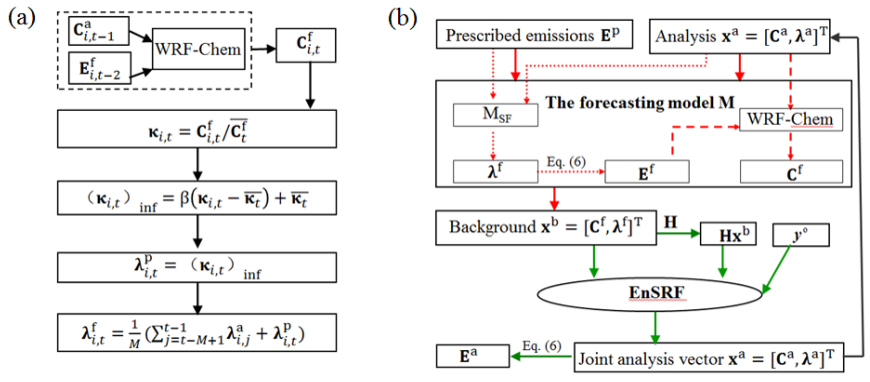
\includegraphics[width=30pc,angle=0,scale=2.5]{figure/Methodology.png}}
                    \caption{(a) describe the framework to integrate scaling factor $\lambda$. (b) flow chart of the data assimilation system that simultaneously optimizes the chemical initial
                    conditions and emissions.}\label{fig2}
                \end{figure}

                % After been integrated and assimilated, the estimated emission $E^a$ can now be calculated by prescribed emission $E^p$ and $\lambda^a$ as:
                % \begin{equation}
                %     E^a=\lambda^a*E^{p} 
                % \end{equation}
				
			
				
			\end{block}

            \begin{block}{System settings and Observation}
                \begin{itemize}
					\item \textbf{simulation model}: WRF-Chem version 3.6.1. The model domain, together with Yangtze River Delta(YRD) region are shown in \cref{fig1},  with a horizontal resolution of 18km. GOCART-RACM-KPP is selected as the aerosol-chemical scheme. 

					\item \textbf{assimilation system}: Ensemble Square Root Filter(EnSRF), with forward operator taken from Gridpoint Statistical Interpolation(GSI). 
                    \sepnewparagraph
					\item \textbf{meteorology observation}: NCEP GDAS. All in situ observations and cloud motion vectors are assimilated every 6 hours. 
     
					\item \textbf{surface chemical observation}: MEE in-situ observation of $PM_{2.5}, PM_{10}, SO_2, NO_2, O_3, CO$. A subset of 560 stations is selected to be assimilated, in order to avoid correlated observations. There are 95 validation station in YRD region. Details of station distribution can be seen in \cref{fig1}.
     

     
				\end{itemize}
                \begin{figure}
                    \centerline{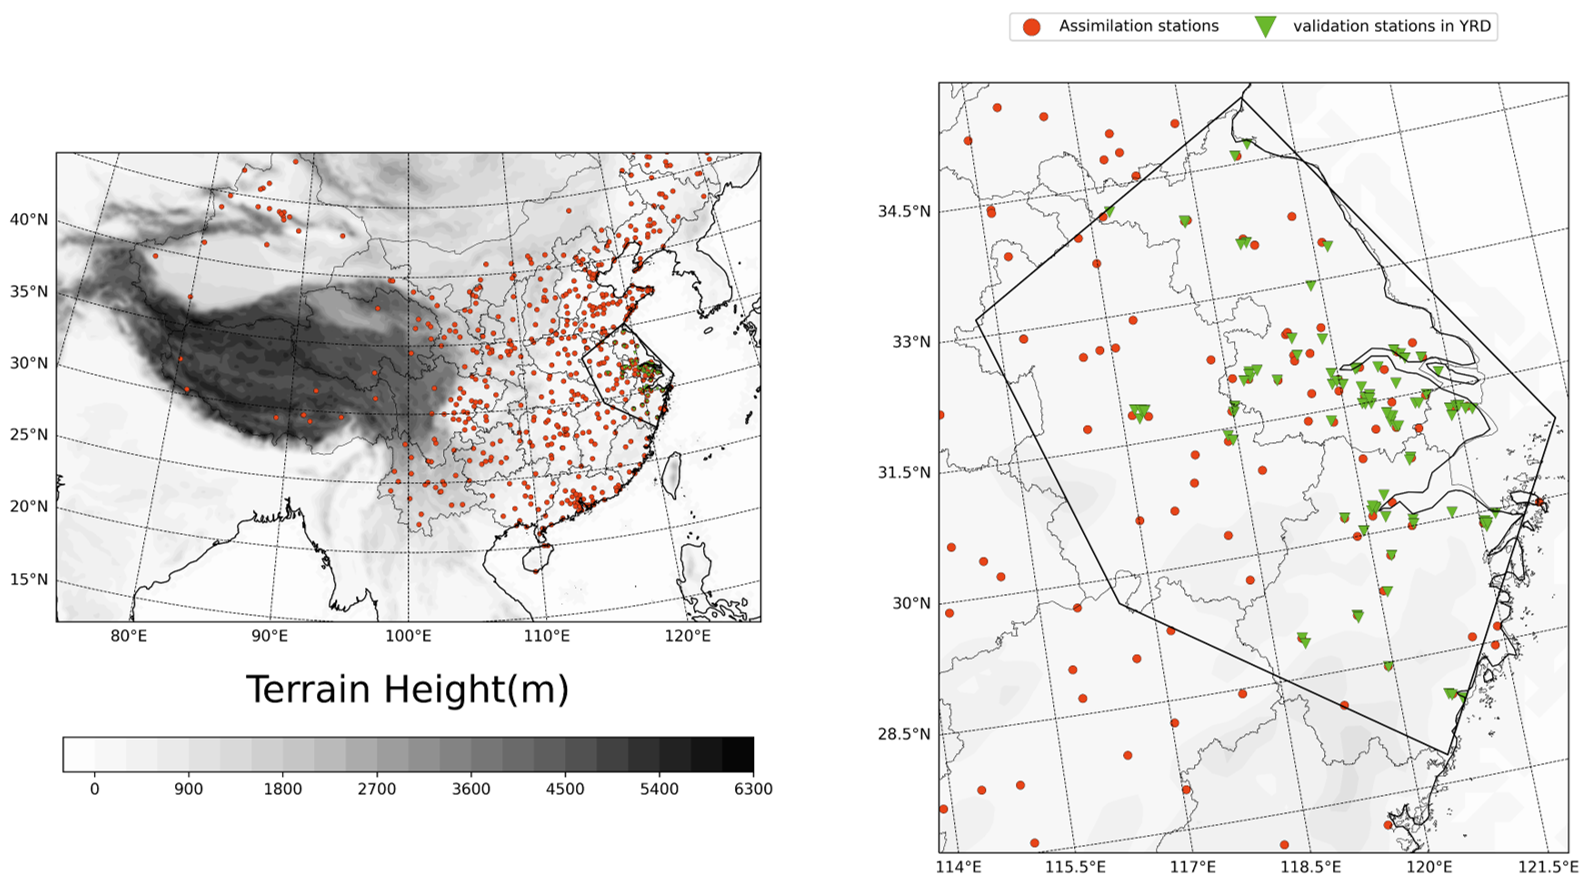
\includegraphics[width=0.9\colwidth,angle=0]{figure/domain_station_split.pdf}}
                    \caption{Domain setting and station distribution. The left subplot shows model domain in WRF-Chem, the shading indicates the terrain height. Red rots represent assimilation stations, and green triangles are validation stations in Yangtze River Delta(YRD) region selected by the black polygon. The right subplot shows more detailed station distribution in YRD region.  }\label{fig1}
                \end{figure}

			\end{block}
   
			\begin{block}{Quantified selection for VOC species}

				

                \begin{wrapfigure}{c}{0.72\colwidth}

                    \centerline{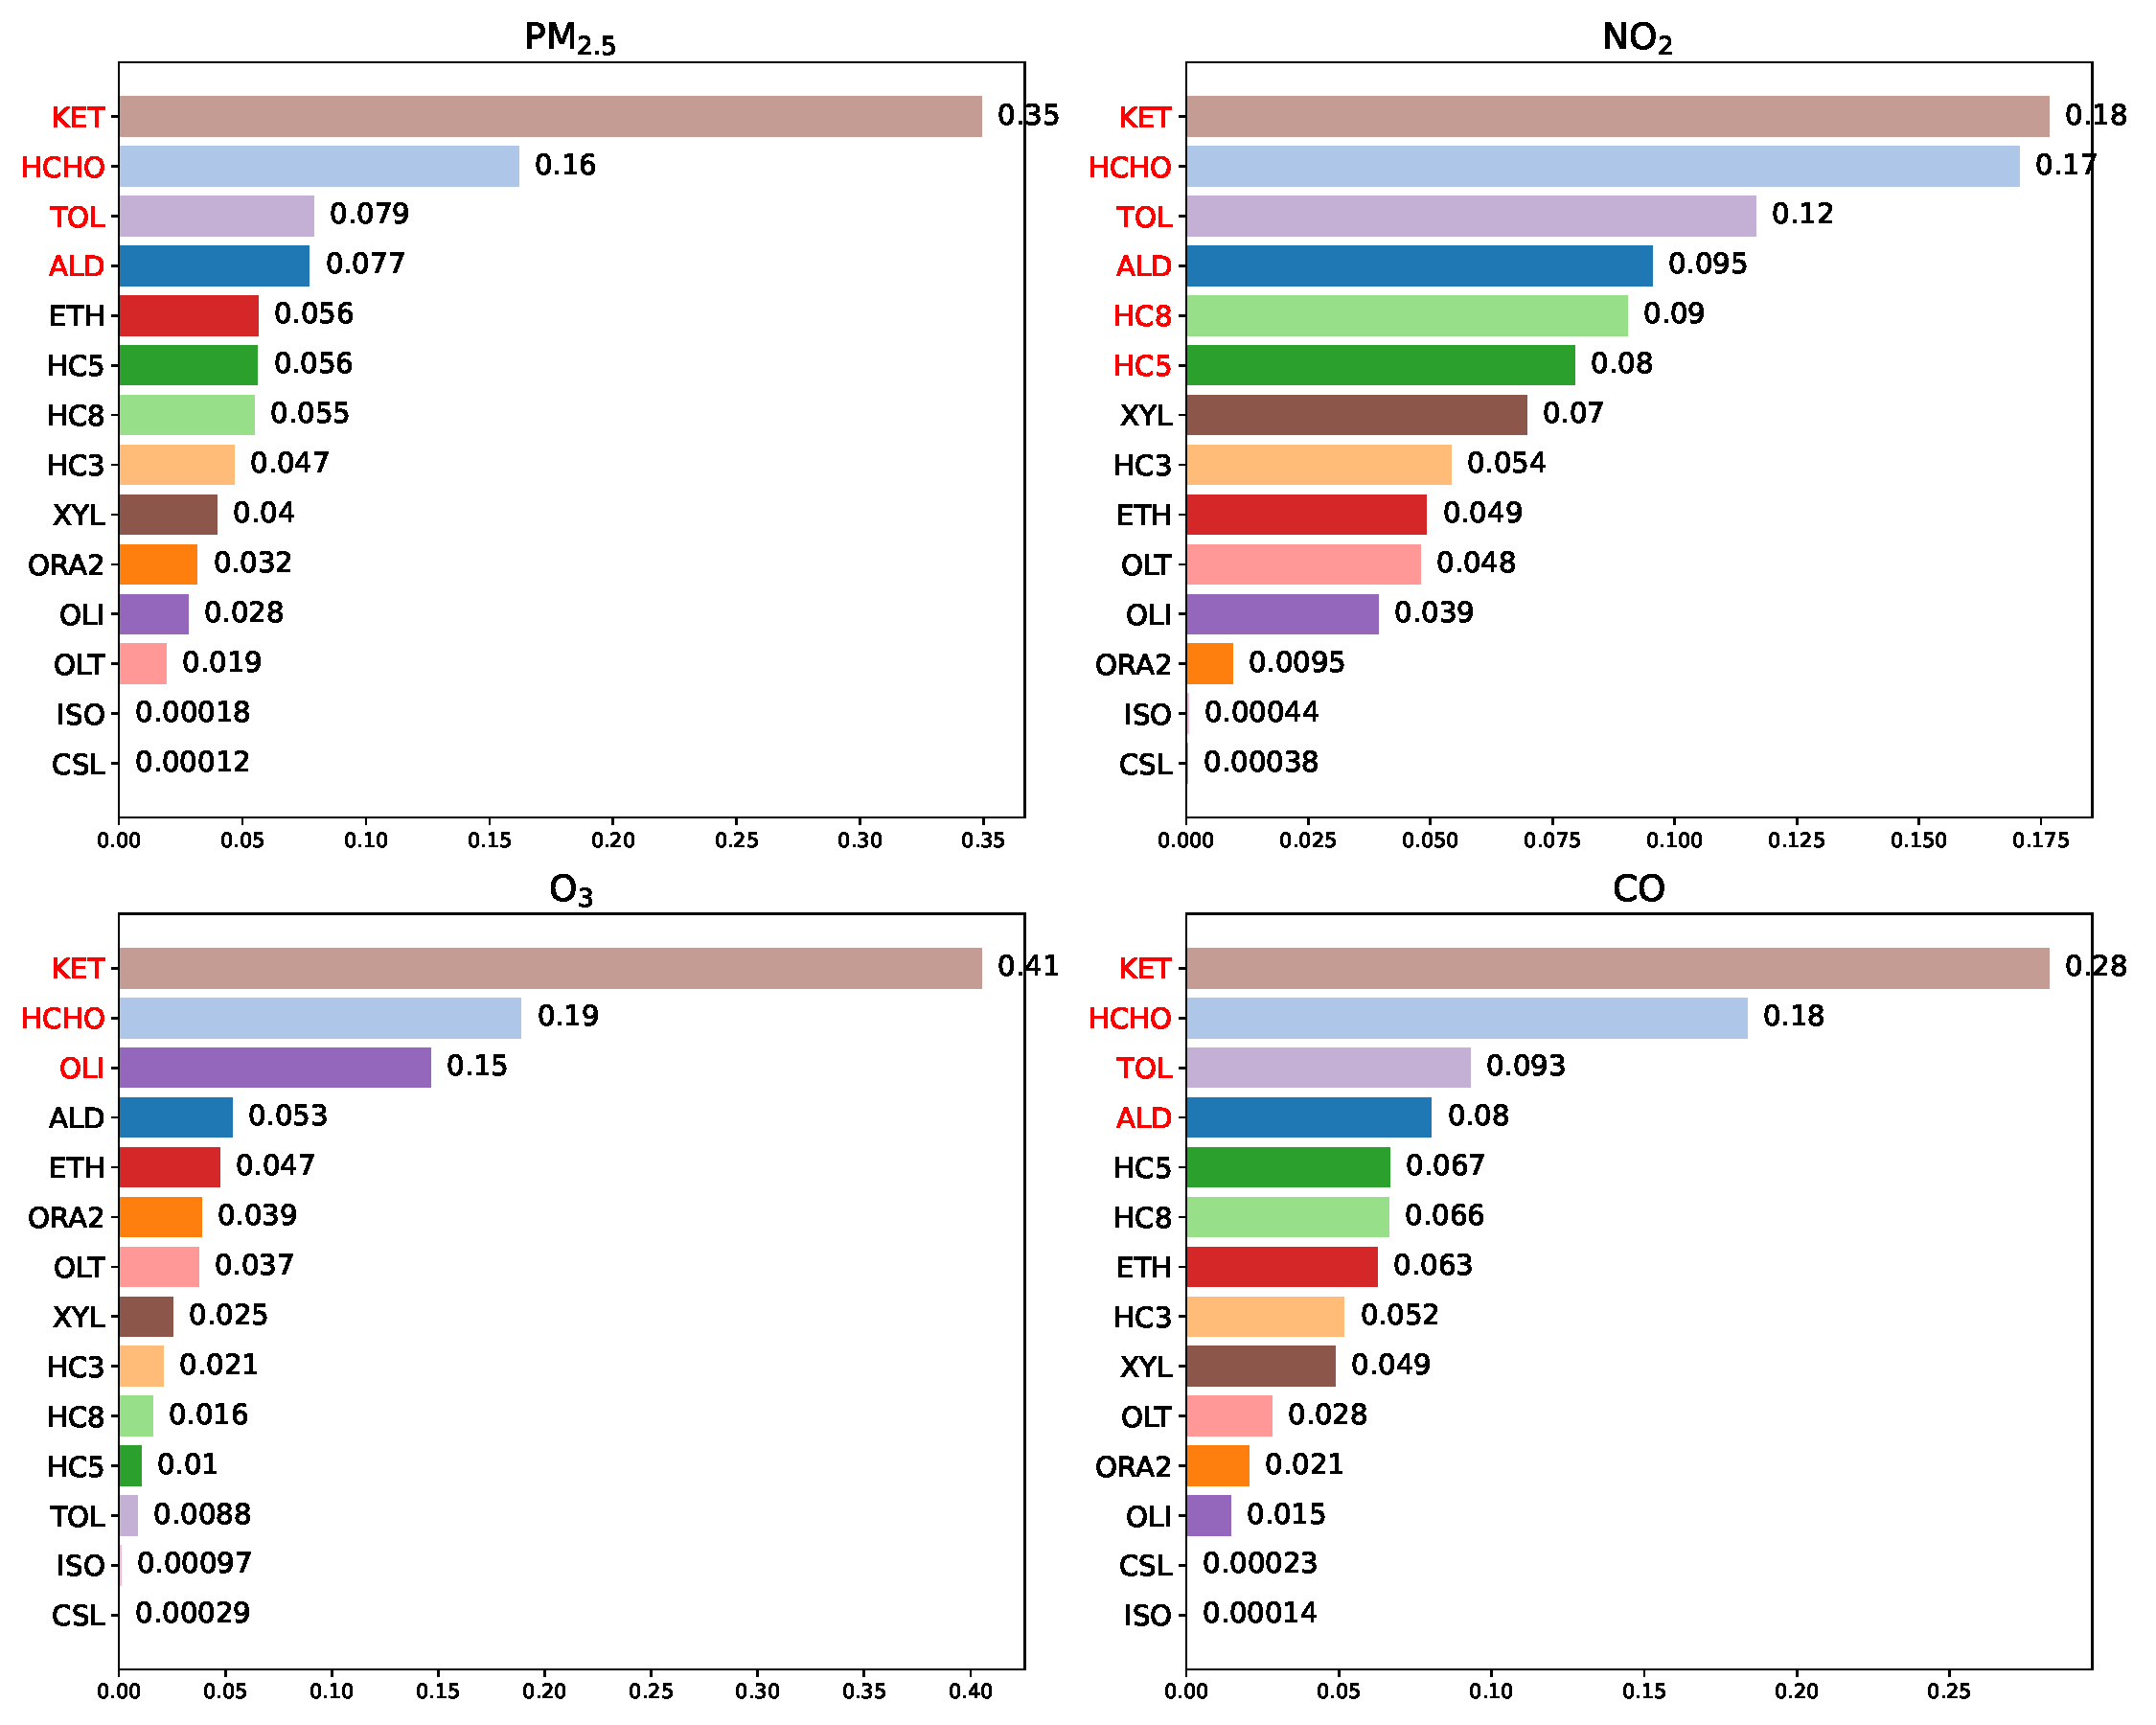
\includegraphics[width=0.7\colwidth,angle=0]{figure/VOC_factor_domainavg.pdf}}                  

                    \caption{Normalized VOC factor for each observation kind. VOCs with a red name will be included in our assimilation system.}   
                    \label{fig_voc_factor}
                \end{wrapfigure}

                \RaggedRight
                A quantified standard will make it clear to decide which VOC species should be updated by observations. Here, we propose a VOC factor to quantify which VOC species should be included in the assimilation system. The VOC factor considers two parts:
                \sepnewparagraph
                \begin{itemize}
                    \item The correlation between observation and VOC species.
                    \item The potential influence of updating VOC species on other variables.
                \end{itemize}
                \sepnewparagraph
                A 50-member ensemble of free forecasts without any assimilation is conducted from 2022-07-10:00 to 2022-08-10:00 to calculate the VOC factor(also provide spin-up IC for cycling assimilation). The potential influence of updating a VOC species is roughly quantified by prescribed emission and average concentration during free forecast period. More details can be found by scan the QR code in Appendix.

			\end{block}

		\end{column}
	
		\separatorcolumn
		
		\begin{column}{\colwidth}
			
			\begin{block}{Experiment design}
               Four experiments are designed to explore the effects of VOC selection for emission estimates: \texttt{NOVOC, O\textsubscript{3}\_AllVOC, O\textsubscript{3}\_CSVOC, AllOBS\_CSVOC}. \\
               
               \sepnewparagraph
               
               A cycling assimilation system is launched for each experiment from 2022-07-20:00 to 2022-07-30:00. The assimilation cycle period is 6h for meteorology variables and 1h for chemical variables/scaling factors. The meteorology variables and six main pollutions, together with their corresponding scaling factors, will be updated in all experiments, which is the same in \parencite{Peng_2020}. The difference between four experiments is the strategy to update VOC species, which is shown in the table below. \\

                \begin{table}[t]

                    \begin{center}
                    \begin{tabular}{l@{\hskip 2\sepwidth}l@{\hskip 2\sepwidth}l}
                    \hline
                    \hline
                    \vspace{0.5em}
                    \textbf{Experiment} & \textbf{Observation} & \textbf{VOC species to be updated} \\
                    \vspace{0.5em}
                    NOVOC & N/A & N/A \\
                    \vspace{0.5em}
                    O\textsubscript{3}\_AllVOC & O\textsubscript{3} & All VOC species \\
                    \vspace{0.5em}
                    O\textsubscript{3}\_CSVOC & O\textsubscript{3} & KET/HCHO/OLI \\
                    AllOBS\_CSVOC & O\textsubscript{3} & KET/HCHO/OLI \\
                     & PM\textsubscript{2.5} & KET/HCHO/OLI \\
                     & NO\textsubscript{2} & KET/HCHO/TOL/ALD/HC8/HC5 \\
                     & CO & KET/HCHO/TOL/ALD \\
                    \hline
                    \end{tabular}
                    
                    \end{center}
                    \caption{Description of VOC selections for each experiment. The VOC species and corresponding scaling factors in the 3rd column will be updated by observations in the 2nd column.}\label{tab_voc}
                    
                \end{table}
                
               Since there is no direct emission observations, the estimated emissions will be evaluated by launching series of 72h forecasts. Starting at 2022-07-22:00, every 6h a deterministic forecast is launched with ensemble mean of cycling analysis as IC and emission estimates of last day as emission input. \\
               \sepnewparagraph
               It should be noted that all kinds of chemical observations have already been used to update their corresponding state variables, thus no new observation is introduced into assimilation system to update VOC species.

			\end{block}

			\begin{alertblock}{Emission estimates}
                \begin{figure}
                \begin{minipage}[c]{0.8\textwidth}
                    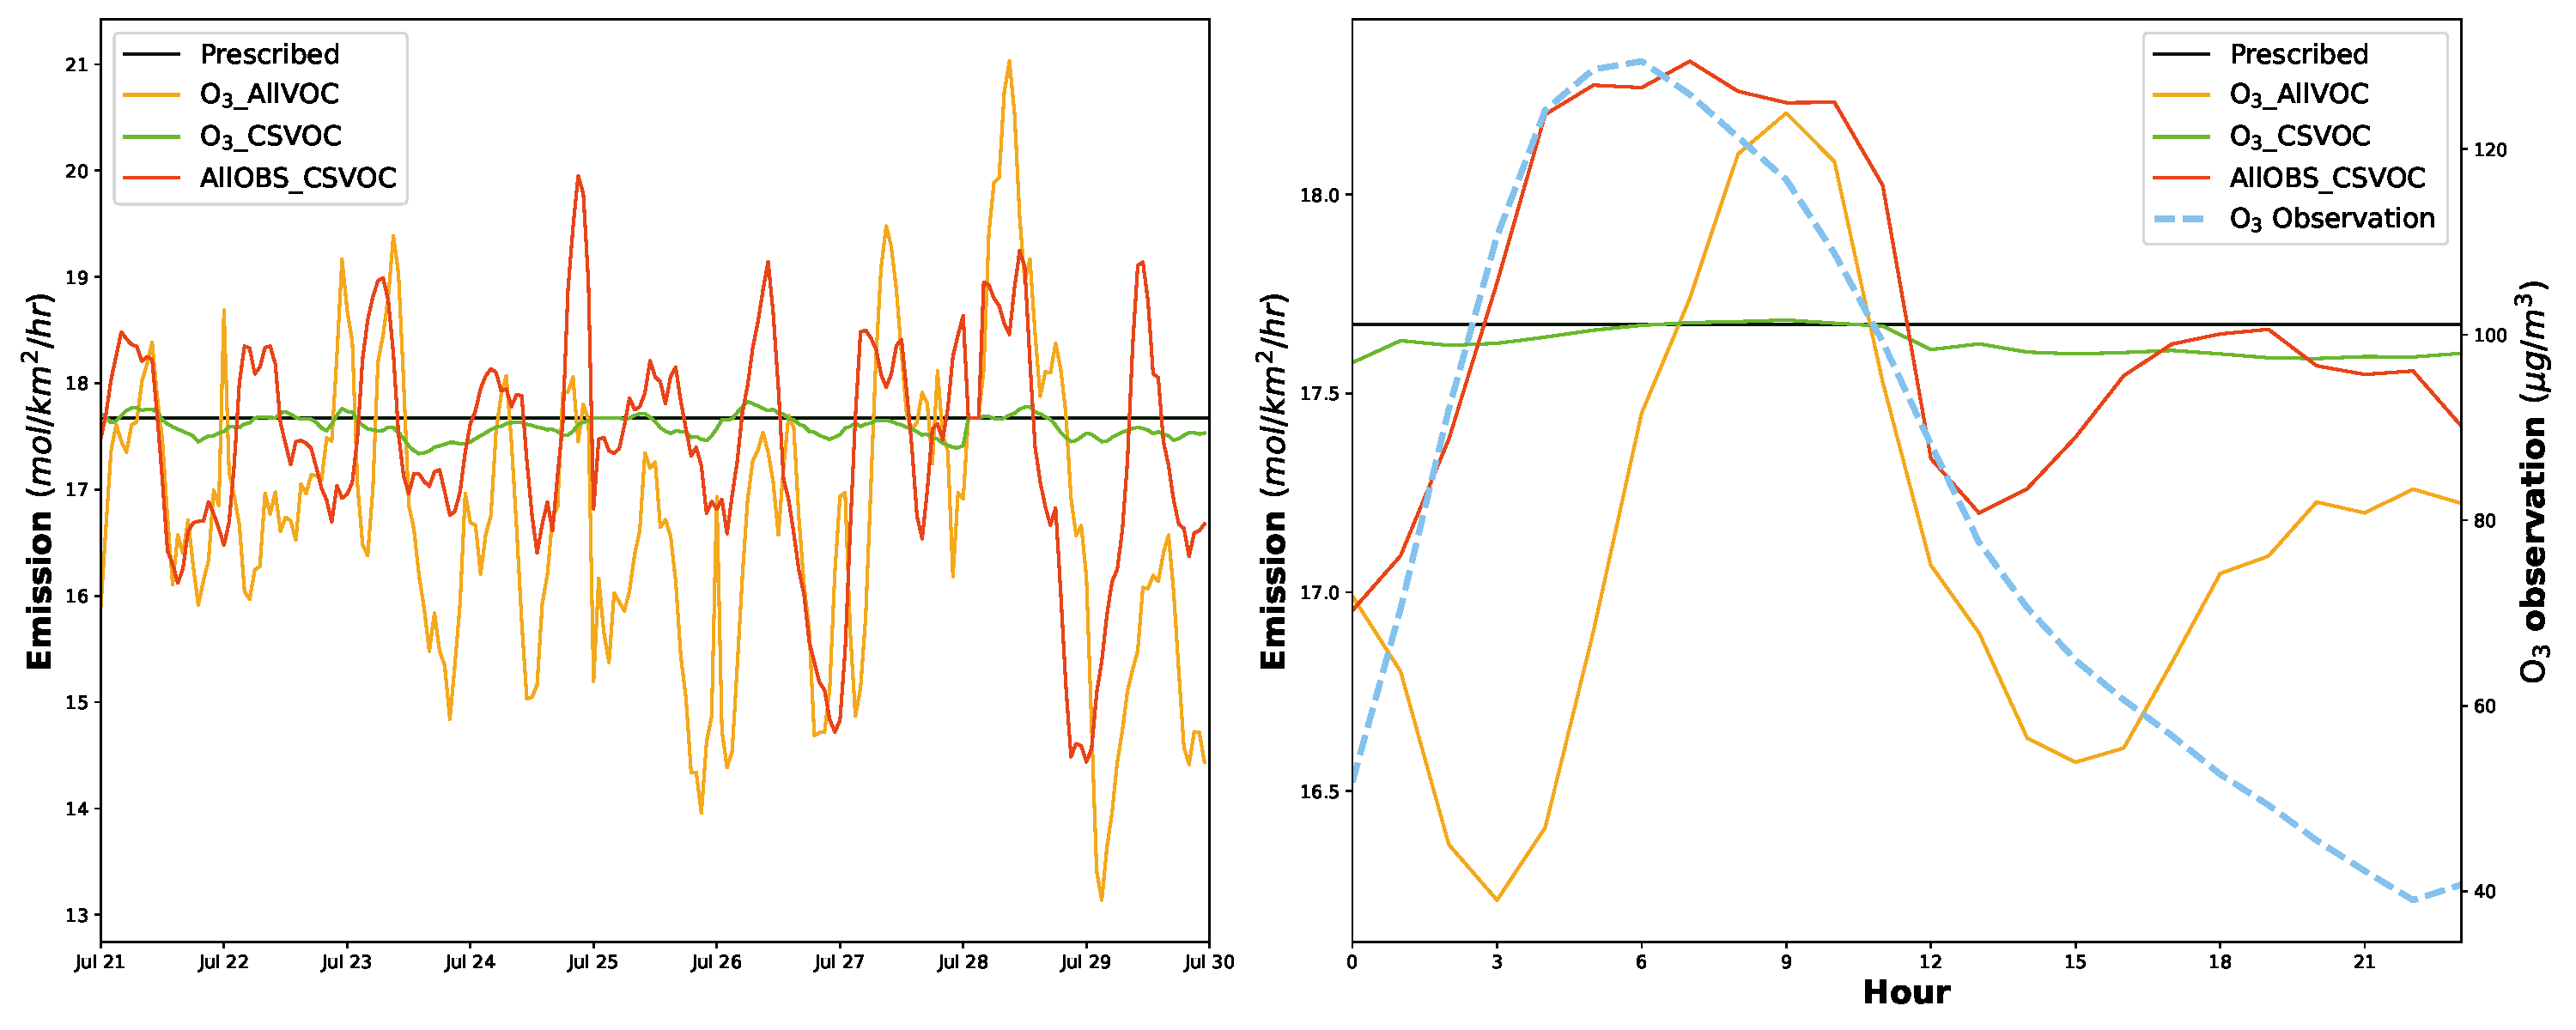
\includegraphics[width=\textwidth]{figure/emiss_ts_diurnal_witho3.pdf}
                \end{minipage}
                \hfill
                 \begin{minipage}[c]{0.18\textwidth}
                    \RaggedRight
                    \caption{The left subplot shows time series of overall VOC emission estimates in each experiment. The right subplot presents diurnal-variation of overall VOC emission estimates in left y-axis, and diurnal-variation of O\textsubscript{3} observation  in right y-axis.}\label{fig_emiss_ts}                     
                 \end{minipage}   

                    
                \end{figure}
                
                \begin{itemize}
                    \item O\textsubscript{3}\_AllVOC estimates have an obvious diurnal variation, but show a suspicious drop in UTC00-UTC03.
                    \item O\textsubscript{3}\_CSVOC estimates fix the suspicious drop in UTC00-UTC03, but present little diurnal variation. This is because only 3 VOC emissions are updated in this experiment, others remain unchanged compared to the prescribed emissions.
                    \item AllOBS\_CSVOC estimates also show an obvious diurnal variation, with a constant peak in daytime. This variation in daytime is similar to the YRD averaged O\textsubscript{3} observation. As important precursors of O\textsubscript{3}, this peak in daytime could help the model to overcome the underestimation  of O\textsubscript{3}, as show in in \cref{fcst_result}.
                \end{itemize}

			\end{alertblock}

			\begin{alertblock}{72H O\textsubscript{3}/PM\textsubscript{2.5} forecast results}
                % \begin{minipage}{0.7\colwidth}
                % \begin{figure}
                %     \begin{minipage}[c]{0.7\textwidth}
                %         % \centerline{\includegraphics[width=0.7\colwidth,angle=0]{figure/fcst72h_00_6hcycle_nocorr.pdf}}
                %         \includegraphics[width=0.7\colwidth,angle=0]{figure/fcst72h_00_6hcycle_nocorr.pdf}
                %     \end{minipage}
                %     \hfill
                %     \begin{minipage}[c]{0.3\textwidth}
                %     \caption{Averaged RMSE/BIAS value for O\textsubscript{3}(1st column) and PM\textsubscript{2.5}(2nd column). The bars on the rightside in each subplot represent the mean value . Units for all this variables: $\mu g/m^3$}                    
                %     \end{minipage}
                %     \label{fcst_result}    
                % \end{figure}
                % \end{minipage}

                \begin{figure}
                  \begin{minipage}[c]{0.8\textwidth}
                    \includegraphics[width=\textwidth]{fcst72h_00_6hcycle_nocorr.pdf}
                  \end{minipage}\hfill
                  \begin{minipage}[c]{0.18\textwidth}
                    \caption{Averaged RMSE/BIAS value for O\textsubscript{3}(1st column) and PM\textsubscript{2.5}(2nd column). The bars on the rightside in each subplot represent the mean value . Units for all this variables: $\mu g/m^3$}    
                    \label{fcst_result}
                  \end{minipage}
                \end{figure}
                
                \begin{itemize}
                    \item O\textsubscript{3}\_AllVOC(yellow) shows little RMSE/BIAS improvements for O\textsubscript{3} and PM\textsubscript{2.5} forecasts compared with NOVOC(black). 
                    \item O\textsubscript{3}\_CSVOC(green) has obvious improvements in PM\textsubscript{2.5} RMSE/BIAS, but failed to improve O\textsubscript{3} forecasts.
                    
                    \item AllOBS\_CSVOC shows advantage for both O\textsubscript{3} and PM\textsubscript{2.5} forecasts, especially in reducing O\textsubscript{3} BIAS. Possibly because AllOBS\_CSVOC estimates have a constant peak in daytime, which compensates for the underestimation of O\textsubscript{3} and serves as a model error correction.
                \end{itemize}
			\end{alertblock}
   
			\begin{block}{}
			    \begin{figure}
                   \begin{minipage}[c]{0.24\colwidth}
                       
\includegraphics[height=6em]{logos/aerss_logo.png}
                   \end{minipage}
                   \begin{minipage}[c]{0.24\colwidth}
                       \textbf{Reference: }\\
                       
\includegraphics[height=6em]{logos/Reference.png}
                   \end{minipage}
                   \begin{minipage}[c]{0.24\colwidth}
                       \textbf{VOC factor details: }\\
                       
\includegraphics[height=6em]{logos/vocfactor_detail.png}
                   \end{minipage}
                   \begin{minipage}[c]{0.24\colwidth}
                       \textbf{Poster source code:}\\
                       
\includegraphics[height=6em]{logos/source_code.png}
                   \end{minipage}
                \end{figure}

			\end{block}
			
		\end{column}
		
		\separatorcolumn
	\end{columns}
\end{frame}
\end{document}